\documentclass{article}
\usepackage{graphicx} % Required for inserting images
\usepackage{enumitem}
\usepackage{xcolor}
\usepackage{listings}

\setlength{\oddsidemargin}{-0.25in}
\setlength{\topmargin}{-0.5in}
\setlength{\headheight}{0cm}
\setlength{\headsep}{0cm}
\setlength{\textheight}{10in}
\setlength{\textwidth}{7in}
\setlength{\topskip}{0cm}

\begin{document}

\noindent\textbf{ComS 472 - PS5 \quad Due: Oct 13, 2024 \quad Name: Aren Ashlock}

\begin{enumerate}

% ------------------------------------- 1 DONE -------------------------------------

\item \textbf{(6 pts)} (Exercise 6.1) How many solutions are there for the map-coloring problem in Figure 6.1 below? How many solutions if four colors are allowed? Two colors?

\begin{center}
    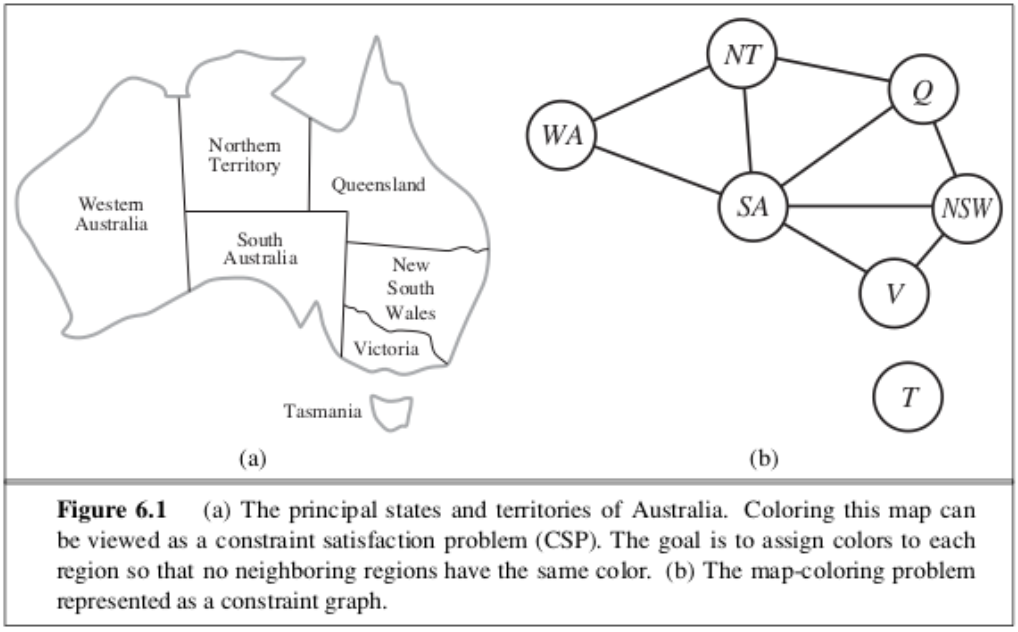
\includegraphics[scale=0.5]{472-PS5-Q1.png}
\end{center}

\color{blue}
    Solutions $= 3*2*1*1*1*1*3 = 18$\\
    Solutions (for 4 colors) $= 4*3*2*2*2*2*4 = 768$\\
    Solutions (for 2 colors) = None
\color{black}

% ----------------------------------------------------------------------------------

% ------------------------------------- 2 DONE -------------------------------------

\item \textbf{(10 pts)} (Exercise 6.5) Solve the cryptarithmetic problem in Figure 6.2 on the next page by hand, using the strategy of backtracking with forward checking and the MRV and least-constraining-value heuristics.

\begin{center}
    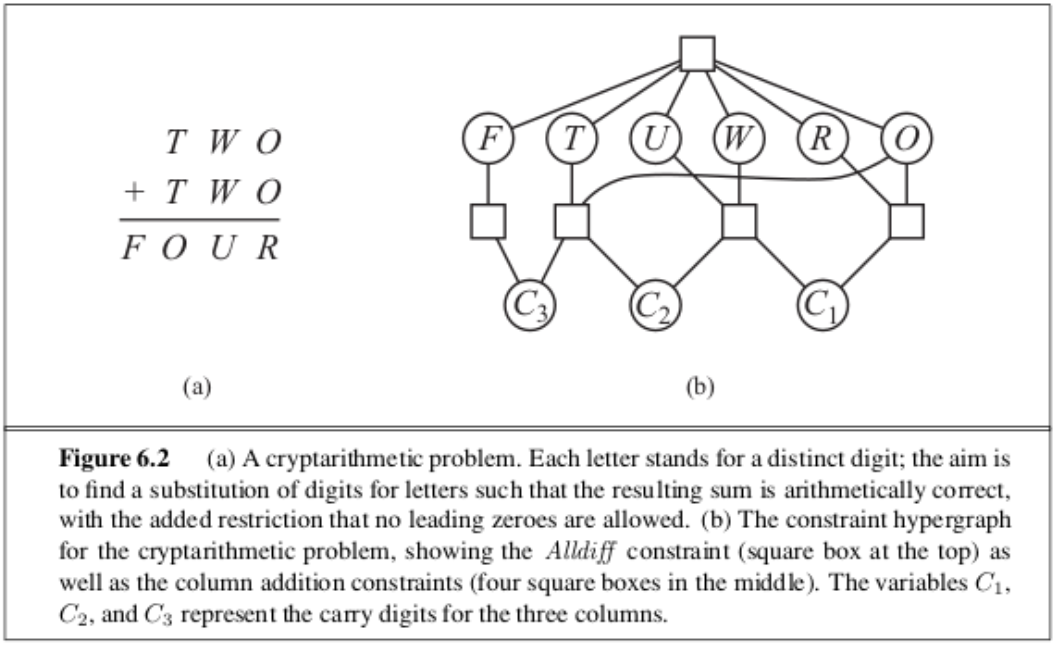
\includegraphics[scale=0.5]{472-PS5-Q2.png}
\end{center}

\color{blue}
    1. Choose $F$ since the domain is $\{1\}$ (MRV), so $F = 1$.\\
    2. Then choose $T$ since the domain is $\{2-9\}$ (MRV), which we have $C_2 + 2T = O + 10 * C_3$, and we know $C_3 = 1$ since $C_3 = F$. This reduces to $C_2 + 2T - 10 = O$. Using least-constraining-value, we can chose $\{6-9\}$ since any the other values result in impossible values for $O$. So, try $T = 6$.\\
    3. By choosing $T = 6$, that reduces the domain of $O$ to $\{2, 3\}$ (MRV), since $C_2 + 2 = O$. Checking for the least-constraining-value, we can see $2O = R + 10 * C_1$. $C_1 = 0$ since it being 1 would result in a negative number. Either value in the domain works in this case, so choose $O = 2$, which also means $C_2 = 0$.\\
    4. Since we chose $O = 2$, the domain of $R$ is only $\{4\}$ (MRV), so we have to choose $R = 4$.\\
    5. The domains of the last 2 letters are the same $\{0, 3, 5, 7, 8, 9\}$, so find a value for $U$. To try and find the least-constraining-value, this equation exists: $2W = U$. The only value that could work would be 8 since $U$ needs to be an even number due to the equation. So choose $U = 8$.\\
    6. The final letter, $W$, has no valid options since the only value that satisfies $2W = U$ since $R = 4$. Therefore, we must backtrack, which we have to backtrack all the way back to $O$.\\
    7. Now we have $F = 1$, $T = 6$, and now we choose $O = 3$ (since it is the only other value in the domain), which means $C_2 = 1$.\\
    8. However, choosing $O = 3$ results in no options for $R$. This is because our equation is now $6 = R + 10 * C_1$, which means the only option for $R$ is 6. But, we already chose $T$ as 6, so we have to backtrack further to $T$.\\
    9. The domain for $T$ was $\{6-9\}$, so we can now try $T = 7$.\\
    10. Reanalyzing $O$ for the least-constraining-value, we have the equation $C_2 + 4 = O$. So the new domain is $\{4, 5\}$. Try $O = 4$.\\
    11. $R$ has only 1 value in the domain since $O = 4$, it must mean $R = 8$.\\
    12. For the final letters, the domain is now $\{0, 2, 3, 5, 6, 9\}$. As learned earlier, the equation we must satisfy is $2W = U$, so we can only choose $U = 6$ to have a legal value for $W$.\\
    13. Finally, we reduce the equation down to $2W = 6$, so we assign $W = 3$.\\
    \textbf{Answer:} $F = 1$, $T = 7$, $O = 4$, $R = 8$, $U = 6$, $W = 3$.
\color{black}

% ----------------------------------------------------------------------------------

% ------------------------------------- 3 DONE -------------------------------------

\item \textbf{(9 pts)} (Exercise 6.11) Use the AC-3 algorithm to show that arc consistency can detect the inconsistency of the partial assignment \{\textit{WA = green, V = red}\} for the map-coloring problem shown in Figure 6.1 on the previous page.

\color{blue}
    * I am skipping over the algorithm iterations which have no effect on the domains *\\
    Arc = (SA, WA), $D_i$ = \{red, green, blue\}, $D_j$ = \{green\}, remove green from $D_i$.\\
    Arc = (SA, V), $D_i$ = \{red, blue\}, $D_j$ = \{red\}, remove red from $D_i$.\\
    Arc = (NT, SA), $D_i$ = \{red, green, blue\}, $D_j$ = \{blue\}, remove blue from $D_i$.\\
    Arc = (NT, WA), $D_i$ = \{red, green\}, $D_j$ = \{green\}, remove green from $D_i$.\\
    Arc = (Q, NT), $D_i$ = \{red, green, blue\}, $D_j$ = \{red\}, remove red from $D_i$.\\
    Arc = (Q, SA), $D_i$ = \{green, blue\}, $D_j$ = \{blue\}, remove blue from $D_i$.\\
    Arc = (NSW, Q), $D_i$ = \{red, green, blue\}, $D_j$ = \{green\}, remove green from $D_i$.\\
    Arc = (NSW, SA), $D_i$ = \{red, blue\}, $D_j$ = \{blue\}, remove blue from $D_i$.\\
    Arc = (NSW, V), $D_i$ = \{red\}, $D_j$ = \{red\}, remove red from $D_i$. Since the size of $D_i$ is 0, this shows an arc inconsistency!
\color{black}

% ----------------------------------------------------------------------------------

\end{enumerate}
\end{document}